\documentclass[12pt]{article}
\usepackage[spanish,mexico]{babel}	\selectlanguage{spanish}
\usepackage{graphicx}
\usepackage{amsmath}
\usepackage{wrapfig}
\usepackage[dvipsnames]{xcolor}
\usepackage{float}
\usepackage{multicol}
\usepackage{geometry}
\usepackage{hyperref}
\usepackage[utf8]{inputenc}

\newgeometry{top=2cm}

\title{Actividad 10}
\author{Paulina Valenzuela Coronado}
\date{today}

\begin{document}
\maketitle
\section{Introducción}
En esta actividad recreamos las animaciones del artículo del péndulo en wikipedia\cite{P}, apoyandonos de la biblioteca de matplotlib de Python.
Usamos un ejemplo del Matplotlib Animation Tutorial\cite{A} y lo adaptamos para crear las animaciones antes mencionadas.
En el caso del movimiento en el espacio físico del péndulo, tuvimos que ajustar el código para diferentes velocidades y ángulos de oscilación.

A continuación se presenta el código modificado y una imagen de cada ejemplo.

\section{Código para el movimiento del espacio físico de un péndulo}
\begin{verbatim}
from numpy import sin, cos
import numpy as np
import matplotlib.pyplot as plt
import scipy.integrate as integrate
import matplotlib.animation as animation

#Movimiento Fisico del Pendulo

class DoublePendulum:
"""Double Pendulum Class

init_state is [theta1, omega1, theta2, omega2] in degrees,
where theta1, omega1 is the angular position and velocity of the first
pendulum arm, and theta2, omega2 is that of the second pendulum arm
"""
def __init__(self,
init_state = [ 120 ,0, 0, 0],
L1=1.0,  # length of pendulum 1 in m
L2=0.0,  # largo
M1=1.0,  # mass of pendulum 1 in kg
M2=1.0,  # mass of pendulum 2 in kg
G=9.8,  # acceleration due to gravity, in m/s^2
origin=(0, 0)): 
self.init_state = np.asarray(init_state, dtype='float')
self.params = (L1, L2, M1, M2, G)
self.origin = origin
self.time_elapsed = 0

self.state = self.init_state * np.pi / 180.

def position(self):
"""compute the current x,y positions of the pendulum arms"""
(L1, L2, M1, M2, G) = self.params

x = np.cumsum([self.origin[0],
L1 * sin(self.state[0])])
y = np.cumsum([self.origin[1],
-L1 * cos(self.state[0])])
return (x, y)


def dstate_dt(self, state, t):
#    """compute the derivative of the given state"""
(M1, M2, L1, L2, G) = self.params

dydx = np.zeros_like(state)
dydx[0] = state[1]
dydx[2] = state[3]

cos_delta = cos(state[2] - state[0])
sin_delta = sin(state[2] - state[0])

den1 = (M1 + M2) * L1 - M2 * L1 * cos_delta * cos_delta
dydx[1] = (M2 * L1 * state[1] * state[1] * sin_delta * cos_delta
+ M2 * G * sin(state[2]) * cos_delta
+ M2 * L2 * state[3] * state[3] * sin_delta
- (M1 + M2) * G * sin(state[0])) / den1

return dydx


def step(self, dt):
"""execute one time step of length dt and update state"""
self.state = integrate.odeint(self.dstate_dt, self.state, [0, dt])[1]
self.time_elapsed += dt

return self.state


#------------------------------------------------------------
# set up initial state and global variables
pendulum = DoublePendulum([90, 15, 0., 0.0]) #theta1, omega1, theta2, omega2
dt = 1./30 # 30 fps

#------------------------------------------------------------
# set up figure and animation

fig = plt.figure()
ax = fig.add_subplot(111, aspect='equal', autoscale_on=False,
xlim=(-2, 2), ylim=(-2, 2)) #tamao ejes
ax.grid()

line, = ax.plot([], [], 'o-', lw=2, color='magenta')
time_text = ax.text(0.02, 0.95, '', transform=ax.transAxes)



def init():
"""initialize animation"""
line.set_data([], [])
time_text.set_text('')
return line, time_text


def animate(i):
"""perform animation step"""
global pendulum, dt
pendulum.step(dt)

line.set_data(*pendulum.position())
time_text.set_text('tiempo = %.1f' % pendulum.time_elapsed)
return line, time_text



# choose the interval based on dt and the time to animate one step
from time import time
t0 = time()
animate(0)
t1 = time()
interval = 1000 * dt - (t1 - t0)

ani = animation.FuncAnimation(fig, animate, frames=80,
interval=interval, blit=True, init_func=init)

ani.save('pendulo0', writer='ffmpeg')


plt.show()

##Espacio fase del mal
def pend(y, t, b, c):
theta, omega = y
dydt = [omega, -b*omega - c*np.sin(theta)]
return dydt

b = 0.0 #friccin
g = 9.8 #gravedad
l = 4.5 #longitud de la cuerda
c = g/l


y0 = [(90*np.pi)/180, 15.0] 

t = np.linspace(0, 20, 100) 

from scipy.integrate import odeint
sol = odeint(pend, y0, t, args=(b, c))




#Crear archivo
np.savetxt("90.txt", sol)

file = open("90.txt","r")
print file.read()

import matplotlib.pyplot as plt 
import numpy as np


data = np.loadtxt('90.txt')

x1=data[:,0] #velocidad angular
y1=data[:,1] #posicin angular



x11 = x1.astype(np.float) #velocidad
y11 = y1.astype(np.float) #posicin


#animacion espacio fase

import numpy as np
import matplotlib.pyplot as plt
from matplotlib.lines import Line2D
import matplotlib.animation as animation



class SubplotAnimation(animation.TimedAnimation):
def __init__(self):
fig = plt.figure()
#posicion de los cuadros de animacion
ax1 = fig.add_subplot(1, 1, 1) #plano xy
#ax2 = fig.add_subplot(2, 2, 2) #plano yz
#ax3 = fig.add_subplot(2, 2, 4) #plano xz


#funcin a graficar
self.t = np.linspace(0, 80, 300)
self.x = x11 #np.cos((np.pi/2) * self.t / 10.) #funcion eje x
self.y = y11 #np.sin((np.pi/2) * self.t / 10.) #funcin eje y
self.z = 5 * self.t


#caracteristicas animacion eje xy
ax1.set_xlabel('Posicion angular')
ax1.set_ylabel('Velocidad angular')
self.line1 = Line2D([], [], color='pink')
self.line1a = Line2D([], [], color='magenta', linewidth=2)
self.line1e = Line2D(
[], [], color='magenta', marker='o', markeredgecolor='b')
ax1.add_line(self.line1)
ax1.add_line(self.line1a)
ax1.add_line(self.line1e)
ax1.set_xlim(-4, 4)#tamano eje x
ax1.set_ylim(-8, 8)#tamao eje y
#ax1.set_aspect('equal', 'datalim')


animation.TimedAnimation.__init__(self, fig, interval=115, blit=115)

def _draw_frame(self, framedata):
i = framedata
head = i - 1
head_len = 10
head_slice = (self.t > self.t[i] - 1.0) & (self.t < self.t[i])

self.line1.set_data(self.x[:i], self.y[:i])
self.line1a.set_data(self.x[head_slice], self.y[head_slice])
self.line1e.set_data(self.x[head], self.y[head])

self._drawn_artists = [self.line1, self.line1a, self.line1e,
#self.line2, self.line2a, self.line2e,
#self.line3, self.line3a, self.line3e
]

def new_frame_seq(self):
return iter(range(self.t.size))

def _init_draw(self):
lines = [self.line1, self.line1a, self.line1e,
#self.line2, self.line2a, self.line2e,
#self.line3, self.line3a, self.line3e
]
for l in lines:
l.set_data([], [])

ani = SubplotAnimation()
#ani.save('pendulo0F', writer='ffmpeg')


plt.show()

\end{verbatim}

	
\begin{figure}[H]
	\centering
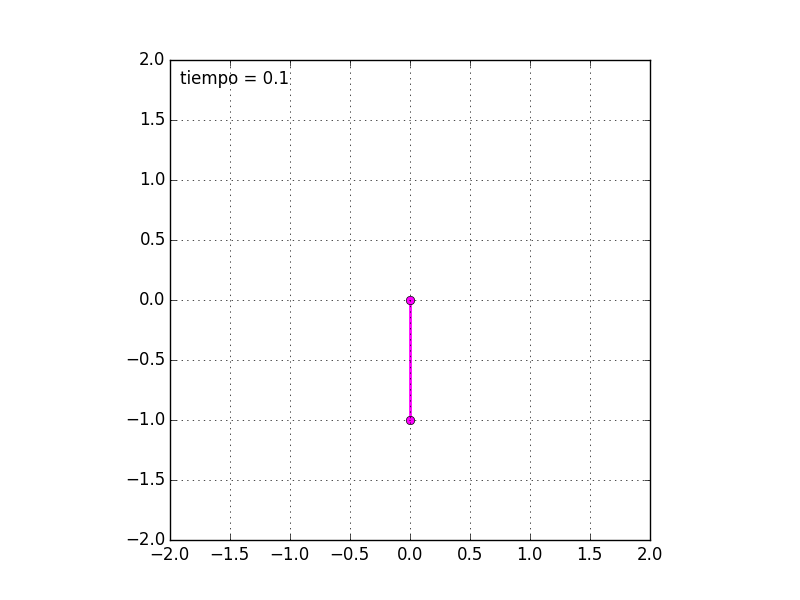
\includegraphics[width=9cm]{0.png}
\caption{0 grados}
\end{figure}

\begin{figure}[H]
		\centering
	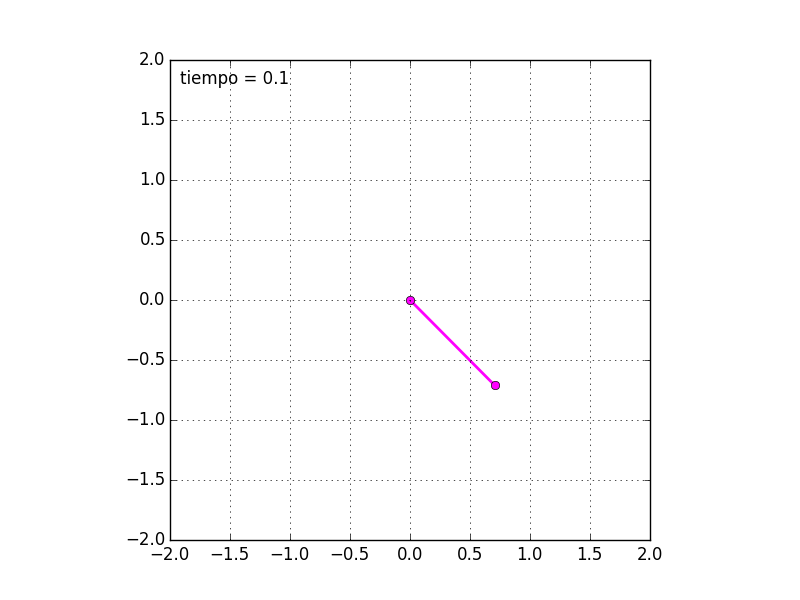
\includegraphics[width=9cm]{45}
	\caption{45 grados}
\end{figure}

\begin{figure}[H]
		\centering
	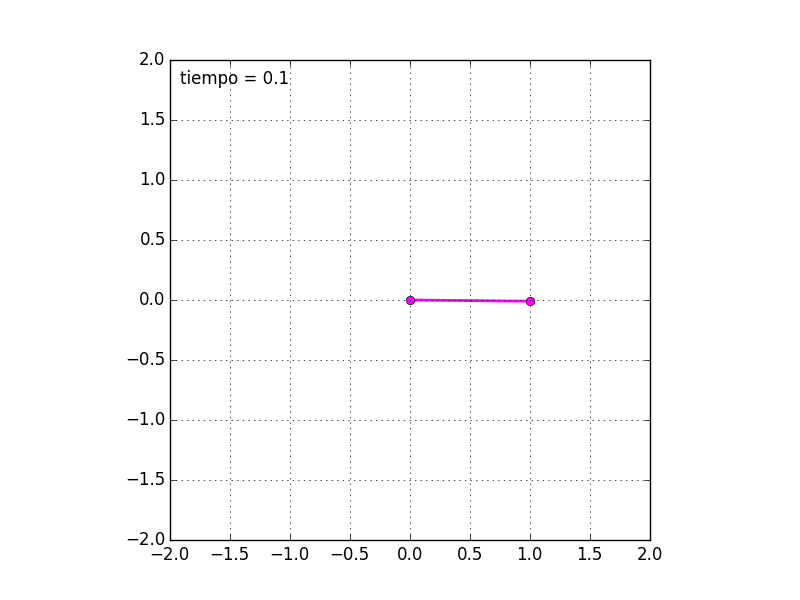
\includegraphics[width=9cm]{90.png}
	\caption{90 grados}
\end{figure}

\begin{figure}[H]
		\centering
	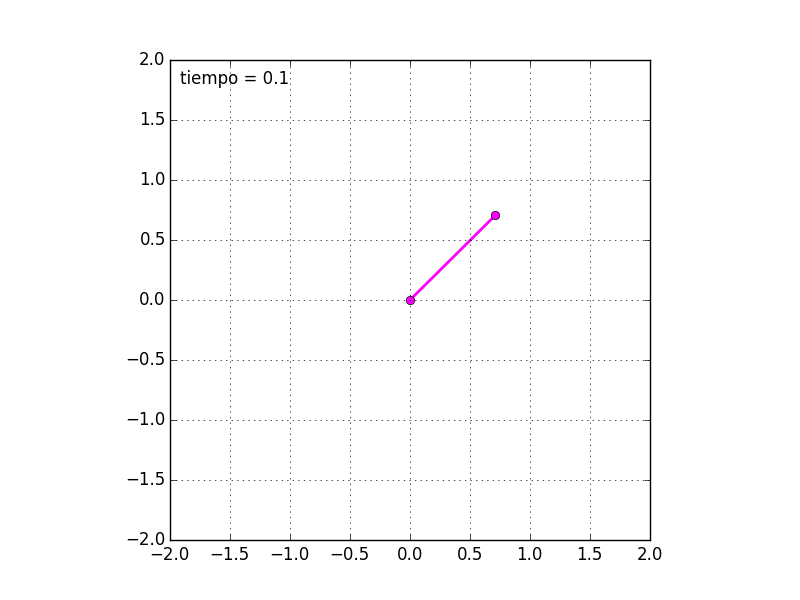
\includegraphics[width=9cm]{135.png}
	\caption{135 grados}
\end{figure}

\begin{figure}[H]
		\centering
	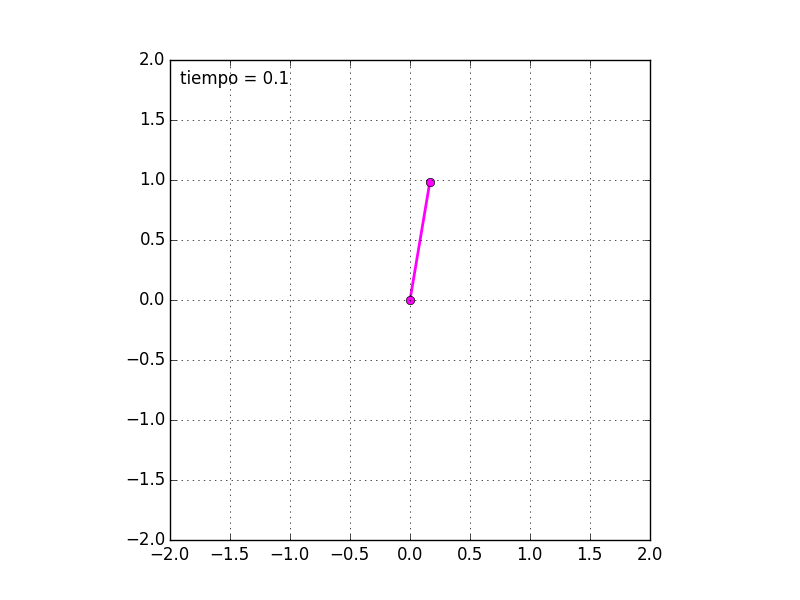
\includegraphics[width=9cm]{170.png}
	\caption{170 grados}
\end{figure}

\begin{figure}[H]
		\centering
	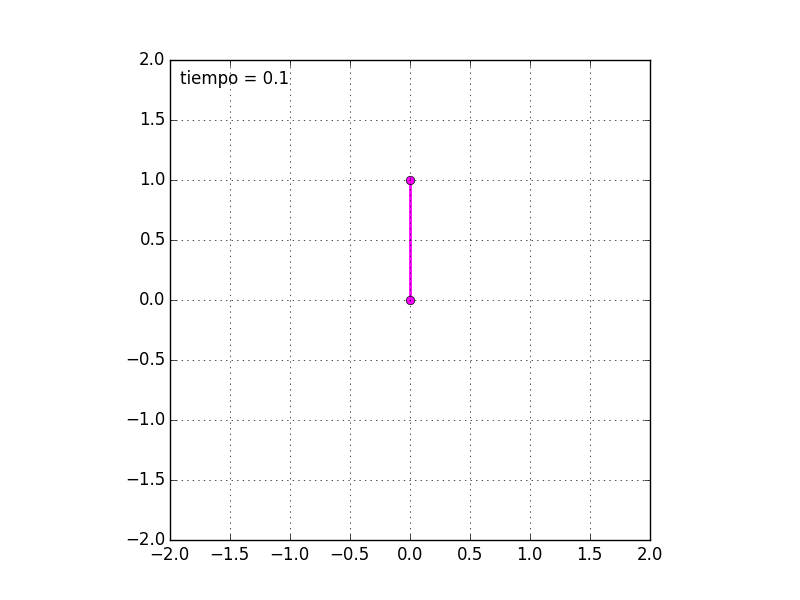
\includegraphics[width=9cm]{180.png}
	\caption{180 grados}
\end{figure}

\begin{figure}[H]
		\centering
	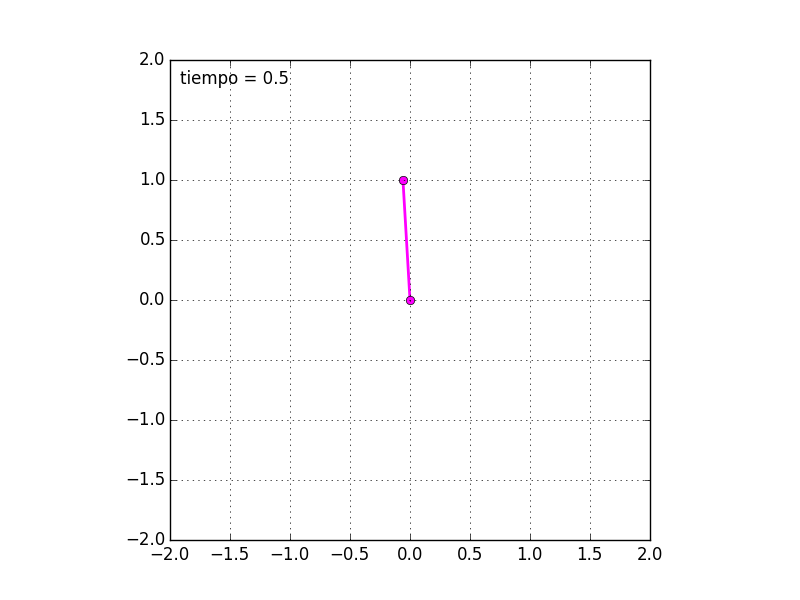
\includegraphics[width=9cm]{j.png}
	\caption{Péndulo con apenas suficiente energía para un ciclo completo}
\end{figure}

\begin{figure}[H]
		\centering
	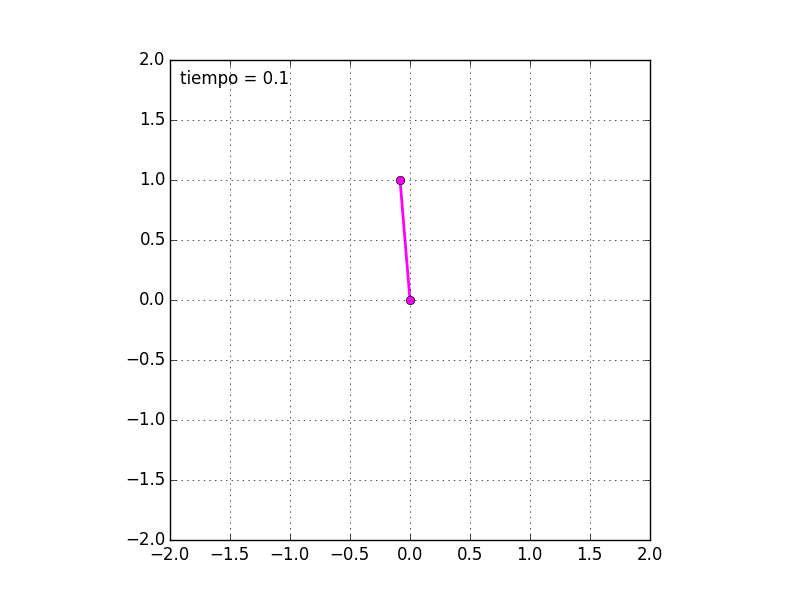
\includegraphics[width=9cm]{s.png}
	\caption{Péndulo con suficiente energía para un ciclo completo}
\end{figure}


\section{Código para el movimiento del espacio fase de un péndulo}




\begin{figure}[H]
		\centering
	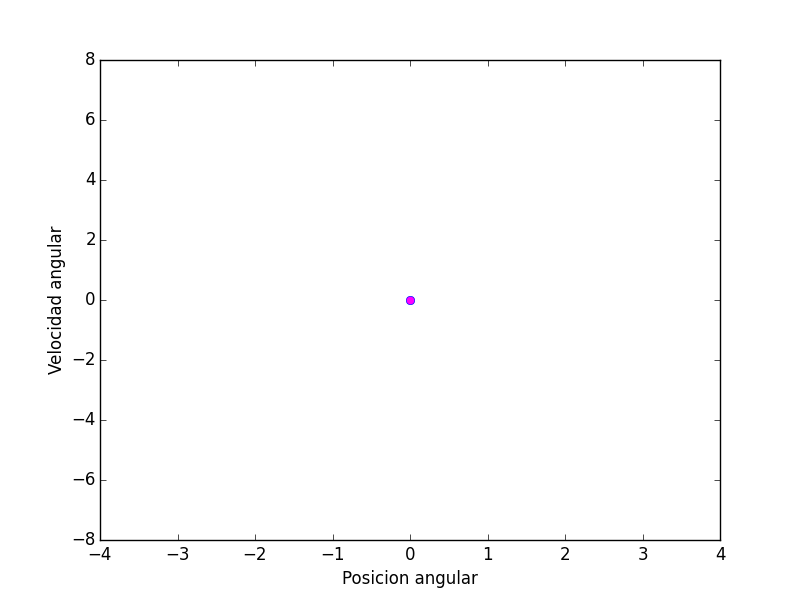
\includegraphics[width=9cm]{0f.png}
	\caption{0 grados}
\end{figure}

\begin{figure}[H]
		\centering
	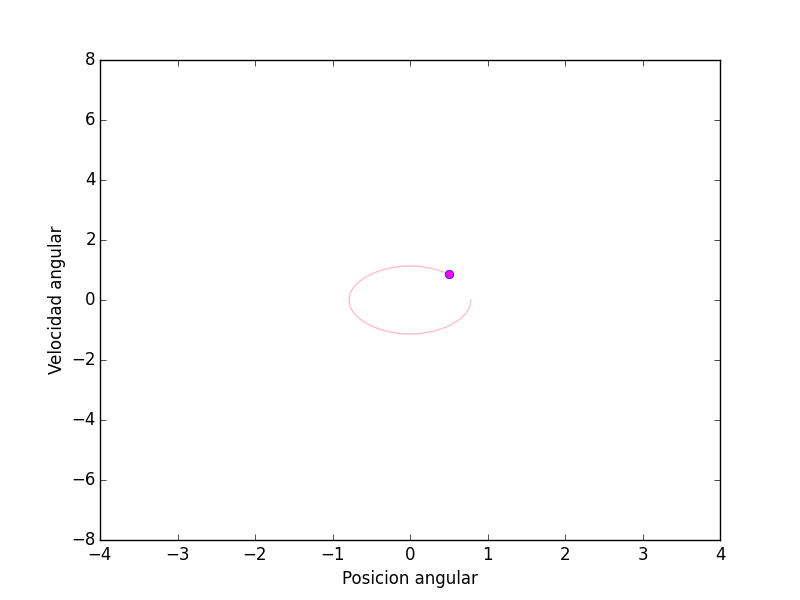
\includegraphics[width=9cm]{45f.png}
	\caption{45 grados}
\end{figure}

\begin{figure}[H]
		\centering
	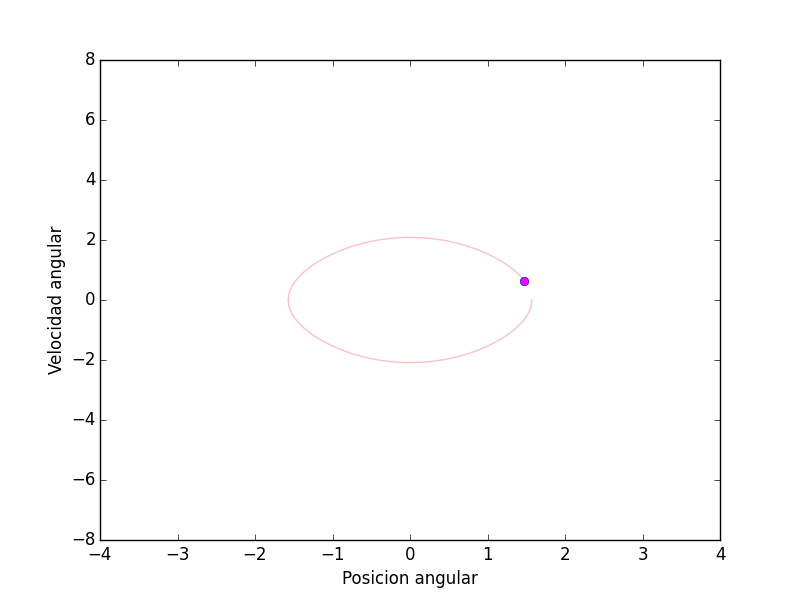
\includegraphics[width=9cm]{90f.png}
	\caption{90 grados}
\end{figure}

\begin{figure}[H]
		\centering
	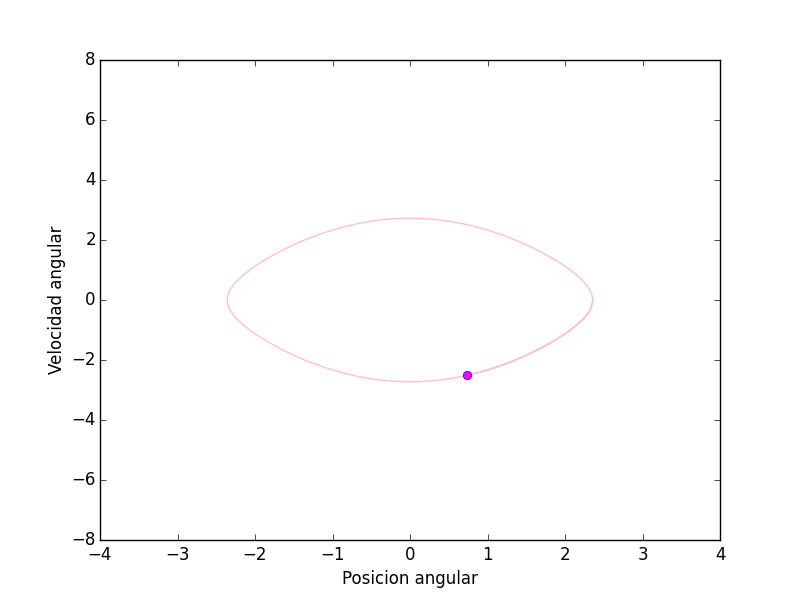
\includegraphics[width=9cm]{135f.png}
	\caption{135 grados}
\end{figure}

\begin{figure}[H]
		\centering
	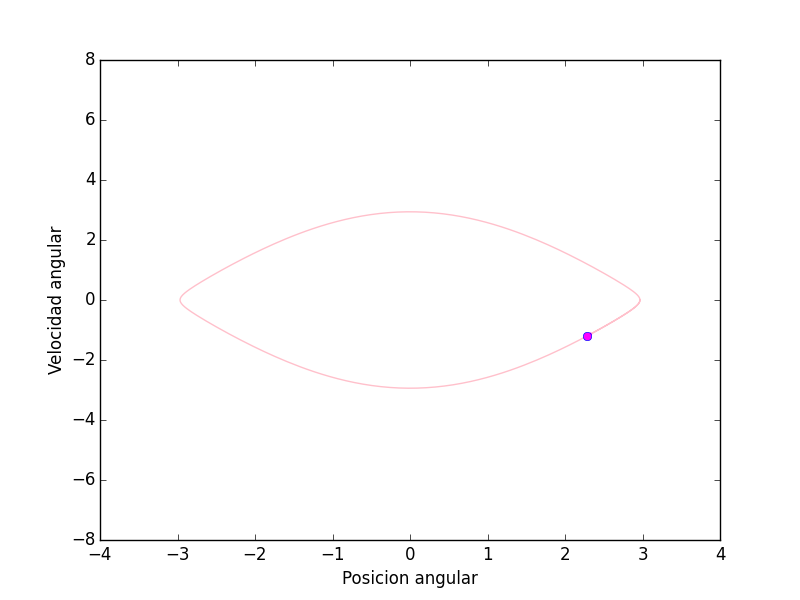
\includegraphics[width=9cm]{170f.png}
	\caption{170 grados}
\end{figure}

\begin{figure}[H]
		\centering
	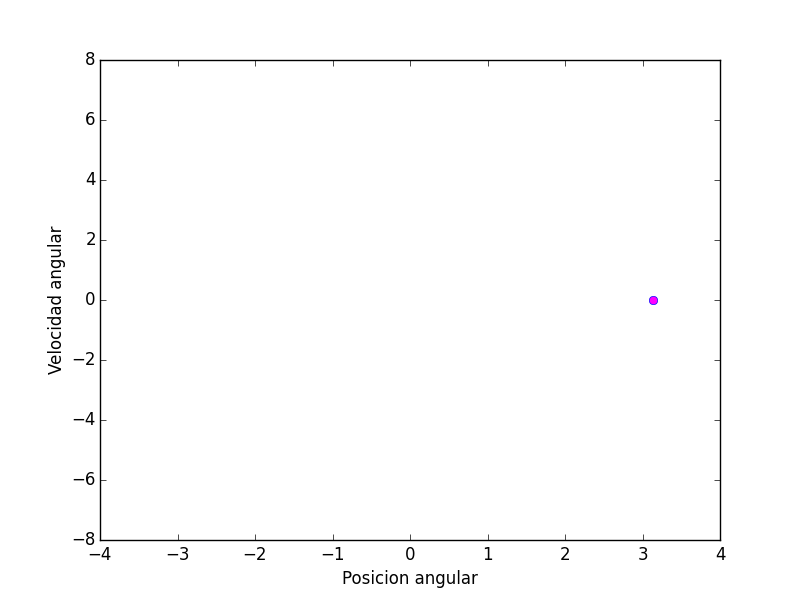
\includegraphics[width=9cm]{180f.png}
	\caption{180 grados}
\end{figure}

\begin{figure}[H]
		\centering
	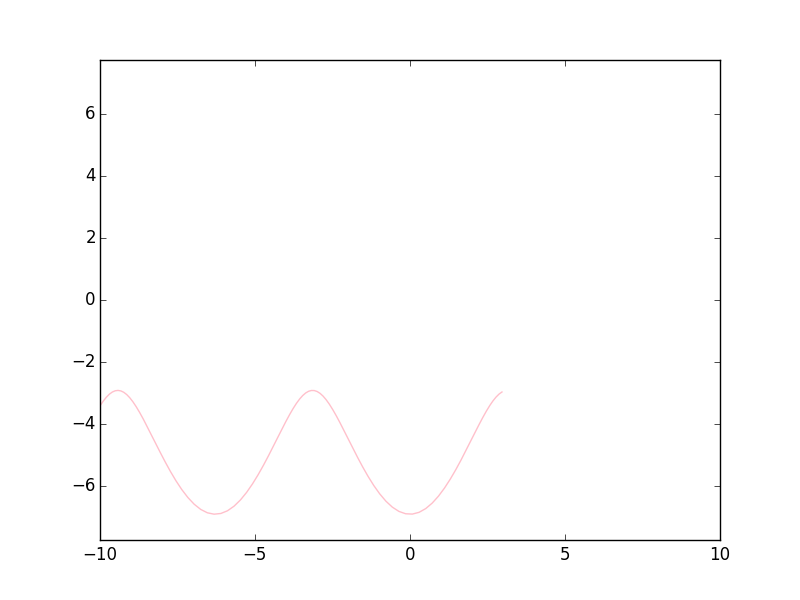
\includegraphics[width=9cm]{jf.png}
	\caption{Péndulo con apenas suficiente energía para un ciclo completo}
\end{figure}







\begin{thebibliography}{6}
	
	\bibitem{P}
	\emph{Péndulo}. 
	\url{https://en.wikipedia.org/wiki/Pendulum_(mathematics)}
	
	\bibitem{A}
	\emph{Matplotlib}. 
	\url{https://jakevdp.github.io/blog/2012/08/18/matplotlib-animation-tutorial/}
	
\end{thebibliography}







\end{document}
